\documentclass{beamer}
\usetheme{Warsaw}

\usepackage[utf8]{inputenc}
\usepackage{fancybox}
\usepackage{multimedia} 
\usepackage{subfig}
\usepackage{amsmath}
\usepackage{hyperref}
\usepackage[all]{xy}
\begin{document}


\title[Digitale Bildverarbeitung] % (optional, only for long titles)
{Digitale Bildverarbeitung
\\
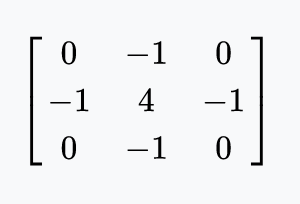
\includegraphics[scale=1.0]{img/cover}
}
\subtitle{}
\author[Dr. Johannes Riesterer] % (optional, for multiple authors)
{Dr.  rer. nat. Johannes Riesterer}

\date[KPT 2004] % (optional)
{}

\subject{Digitale Bildverarbeitung}

\frame{\titlepage}

\begin{frame}
    \frametitle{Einleitung}
\framesubtitle{}
    \begin{block}{Aufgaben der digital Bildverarbeitung}
Operation auf Bildern:
Entrauschen. Entzerren. Kantenerkennung. Segmentierung/Objekterkennung.
\end{block}
    \begin{block}{Anwendungen}
Autonomes Fahren. Gesichtserkennung. Astronomie. Medizin. Ingenieurwesen. Unterhaltungsindustrie. Augmented Reality.
\end{block}
 \end{frame}

\begin{frame}
    \frametitle{Digitale Bilder}
\framesubtitle{}
    \begin{block}{Was ist ein Bild?}
Wir unterscheiden zwischen diskreten und kontinuierlichen Bildern. 
\end{block}

   \begin{block}{Diskretes Bild}
Ein $n$ dimensionales diskretes Bild ist eine Abbildung 
\begin{align*}
U : [1, \ldots, N_1] \times   \cdots \times [1, \ldots, N_n]   \to R
\end{align*}
von $n$ diskreten Intervallen  $[1, \ldots, N_k]  \subset \mathbb{N}$  in einen Farbraum $R$.
\end{block}

   \begin{block}{Kontinuierliches Bild}
Ein $n$ dimensionales kontinuierliches Bild ist eine Abbildung 
\begin{align*}
u : I_1 \times   \cdots \times I_n   \to R
\end{align*}
von $n$ reellen Intervallen $I_k \subset \mathbb{R}$ in einen Farbraum $R$.
\end{block}

 \end{frame}

\begin{frame}
    \frametitle{Digitale Bilder}
\framesubtitle{}
    \begin{block}{RGB Farbraum}
Drei Koordinaten $(R,G,B)$ mit Werten zwischen $(0, 2^{Farbtiefe})$
\end{block}
\begin{figure}[htp]
      \centering
    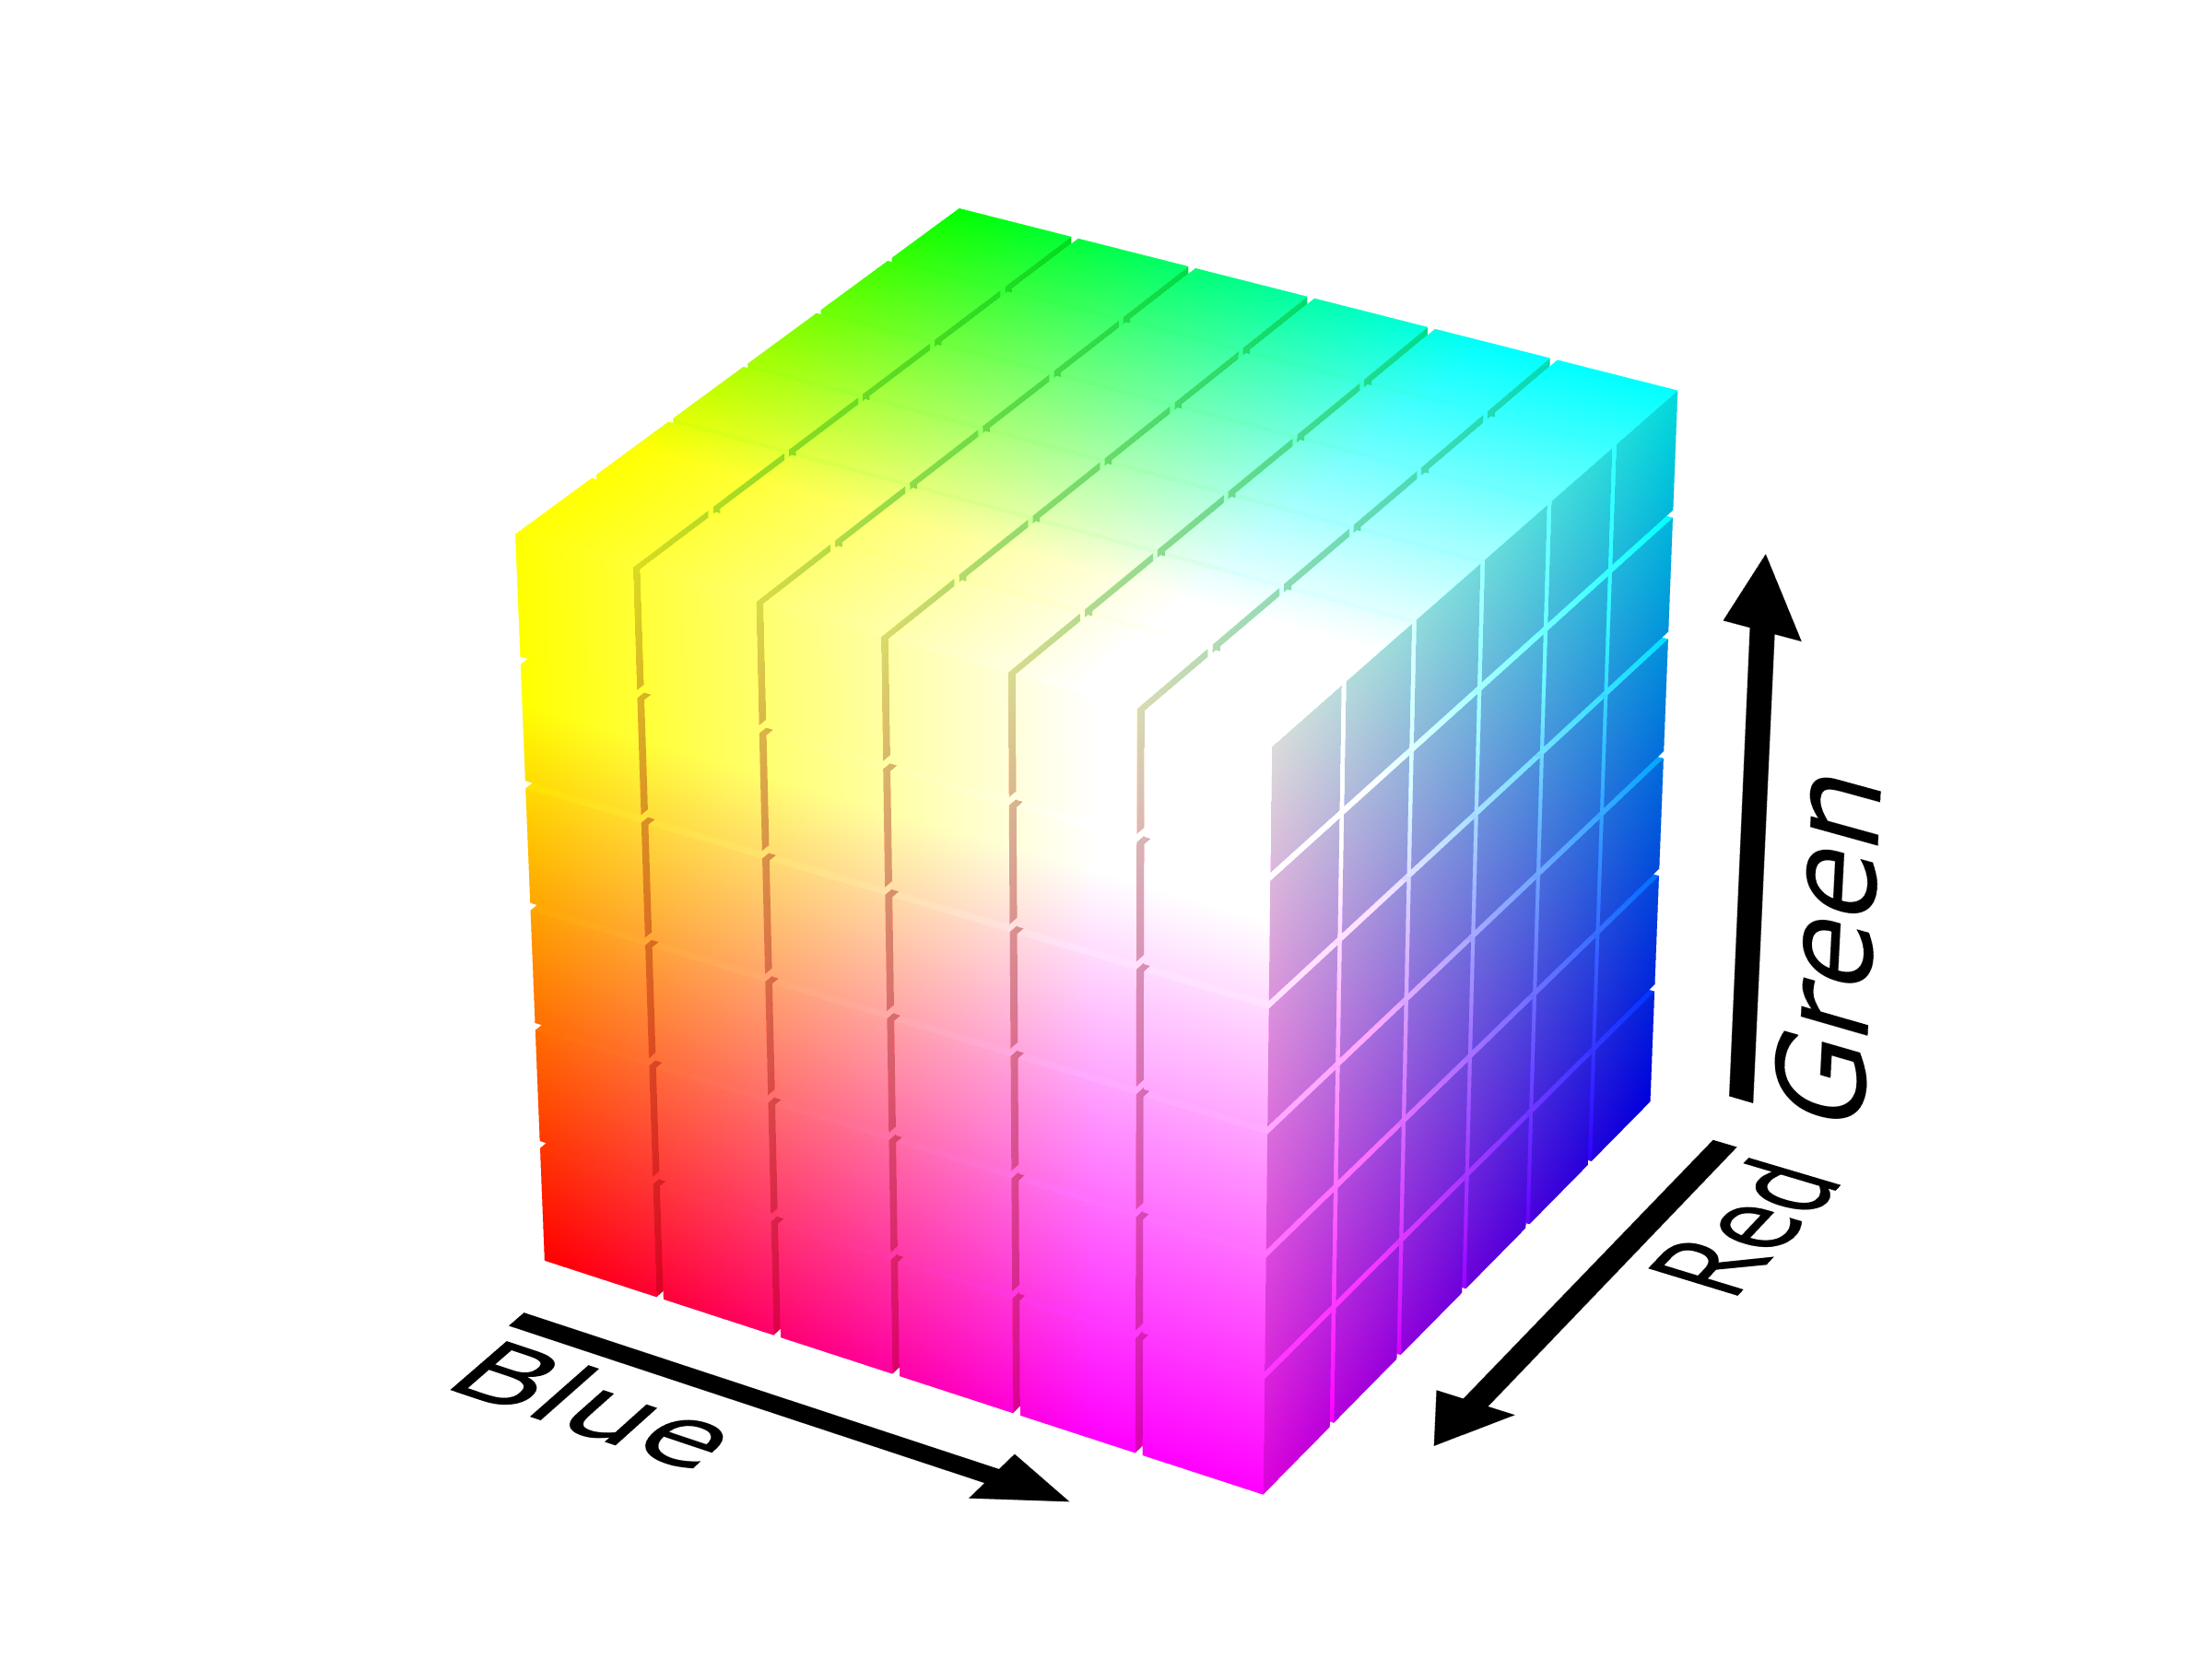
\includegraphics[width=0.45\textwidth]{img/RGB}
      \caption{Quelle: Wikipedia}
\end{figure}

 \end{frame}


\begin{frame}
    \frametitle{Digitale Bilder}
\framesubtitle{}
    \begin{block}{HSV Farbraum}
Drei Koordinaten $(H,S,V)$.
\end{block}
\begin{figure}[htp]
      \centering
    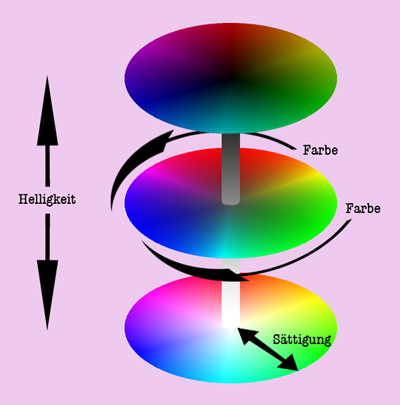
\includegraphics[width=0.45\textwidth]{img/HSV}
      \caption{Quelle: Wikipedia}
\end{figure}

 \end{frame}


\begin{frame}
    \frametitle{Digitale Bilder}
\framesubtitle{}
    \begin{block}{Umwandlung von Bildern}
\begin{itemize}
\item Viele Verfahren der  Signalverarbeitung haben ihren Ursprung in der Analysis. Um diese anwenden zu können, müssen diskrete Daten  in kontinuierliche Daten umgewandelt werden.
\item Auf der anderen Seite kann  ein Computer nur diskrete Daten  verarbeitet. Kontinuierliche Signale (zum Beispiel von Sensoren) müssen daher in diskrete Daten umgewandelt werden.
\end{itemize}
\end{block}

 \end{frame}

\begin{frame}
    \frametitle{Digitale Bilder}
\framesubtitle{}
    \begin{block}{}
Für ein eindimensionales, diskretes Bild $U : [1, \ldots, N]  \to R$ bezeichne  $U_{j} := U(j)$.
\end{block}
    \begin{block}{Stückweise konstante Interpolation}
Definiere $\phi^0 (x) : = 1_{ [-\frac{1} {2} ,  \frac{1} {2}) }(x) : =\begin{cases}
   1 , & \text{for } -\frac{1} {2}  \leq x < \frac{1} {2}  \\
    0  & \text{else } 
  \end{cases} $, $\phi^0_j(x):= \phi^0 (x - j)$ und
 $u(x) := \sum_{j=1}^{N} U_j \phi^0_j(x)$ 
\end{block}

 \end{frame}

\begin{frame}
    \frametitle{Digitale Bilder}
\framesubtitle{}

    \begin{block}{Stückweise lineare Interpolation}
Definiere $\phi^1 (x)  : =\begin{cases}
   x + 1 , & \text{for } -1  \leq x < 0  \\
    1 - x  &  \text{for } 0  \leq x \le 1  \\
 0 &  \text{else} 
  \end{cases}, $ \\ 
$\phi^1_j(x):= \phi^1 (x - j)$ und
 $u(x) := \sum_{j=1}^{N} U_j \phi^1_j(x)$ 
\end{block}

 \end{frame}



\begin{frame}
    \frametitle{Digitale Bilder}
\framesubtitle{}
\begin{block}{Höherdimensionale stückweise  Interpolation}
Für ein 2-dimensionales, diskretes Bild $U : [1, \ldots, N] \times   [1, \ldots, M] \to R$ definiere 
 $u(x, y) := \sum_{i=1}^{N} \sum_{j=1}^{M}  U_{i,j} \cdot \phi_i(x) \cdot \phi_j(y)$ und analog für n-dimensonale Bilder....
\end{block}
 \end{frame}


\begin{frame}
    \frametitle{Digitale Bilder}
\framesubtitle{}
\begin{block}{Abtastung}
Für ein kontinuierliches  Bild $u : I^n \to R$ erhält man durch gewichtete Mittelungen
$U_i := \int_{I^n} \phi (x - x_i) u(x) dx$ ein diskretes Bild. 
\end{block}
 \end{frame}

\end{document}
